\documentclass[a4paper]{article}
\usepackage[T1,T2A]{fontenc}
\usepackage[utf8]{inputenc}
\usepackage[english,russian]{babel}
\usepackage{booktabs}
\usepackage{color,colortbl}
%\usepackage{amsmath}
%\usepackage{amsfonts}
%\usepackage{amssymb}
%\usepackage{makeidx}
\usepackage{listings}
\usepackage{graphicx}
\usepackage{rotating}
\definecolor{green}{RGB}{45,140,31}
\definecolor{darkishgreen}{RGB}{39,203,22}
\definecolor{LightCyan}{rgb}{0.88,1,1}
\definecolor{Gray}{gray}{0.9}
\definecolor{lightRed}{RGB}{230,170,150}
\definecolor{modRed}{RGB}{230,82,90}
\definecolor{strongRed}{RGB}{230,6,6}

\lstset{ %
  language=python,                % Язык программирования
  numbers=left,                   % С какой стороны нумеровать
  extendedchars=\true,
  %numberstyle=tinycolor{gray},     % Стиль который будет использоваться для нумерации строк
  %stepnumber=2,                   % Шаг между линиями. Если 1, то будет пронумерована каждая строка
  %numbersep=5pt,
  %backgroundcolor=color{white},      % Цвет подложки. Вы должны добавить пакет color - usepackage{color}
  showspaces=false,
  showstringspaces=false,
  showtabs=false,
  %frame=single,                    % Добавить рамку
  %rulecolor=color{black},
  tabsize=4,                       % Tab - 2 пробела
  breaklines=true,                 % Автоматический перенос строк
  breakatwhitespace=true,          % Переносить строки по словам
  title=lstname,                   % Показать название подгружаемого файла
  keywordstyle=\color{green},          % Стиль ключевых слов
  %commentstyle=color{dkgreen},       % Стиль комментариев
  %stringstyle=color{mauve}          % Стиль литералов
}

\usepackage[english,russian]{babel}

\title{\bfseriesЛабораторная работа №4.\newline

Разработка клиент-серверного приложения для передачи информации}
\date{}

\begin{document}

\maketitle
\newpage

Цель работы: Научиться реализовывать спрайтовую анимацию в приложениях

\section{Теоретические основы}

Сетевое программирование --- это та его часть, которая подразумевает обмен данными между сервером и клиентом. При этом клиент и сервер --- это не обязательно разные физические сервера, компьютеры, гаджеты. Клиент --- серверная архитектура может быть реализована логически, на одном «железе», в одной комнате, за одним столом. Для взаимодействия между ними используется некоторый свод правил по транспортировке, инкапсуляции, очередности пакетов и сетевого взаимодействия --- это называется протоколом передачи данных. Обычно используют протоколы транспортного уровня TCP и UDP. \textbf{TCP} используют, чтобы формировать между компьютерами двусторонний канал обмена данными. Благодаря TCP пакеты гарантированно доставляются с соблюдением порядка их очередности, с автоматическим разбиением данных на пакеты и контролем их передачи. В то же время TCP работает медленно, так как потерянные пакеты многократно повторно отправляются, а операций, выполняемых над пакетами, слишком много. Протокол \textbf{UDP} --- низкоуровневый. С его помощью компьютеры могут отправлять и получать информацию в виде отдельных пакетов, не создавая логическое соединение. В отличие от TCP, взаимодействия по протоколу UDP не отличаются надежностью. Это усложняет управление ими в приложениях, в которых при обмене информацией нужны гарантии. Поэтому большинство интернет --- приложений используют TCP. Взаимодействие между клиентом и сервером осуществляется с помощью сокета.

\begin{figure}[h]
\center{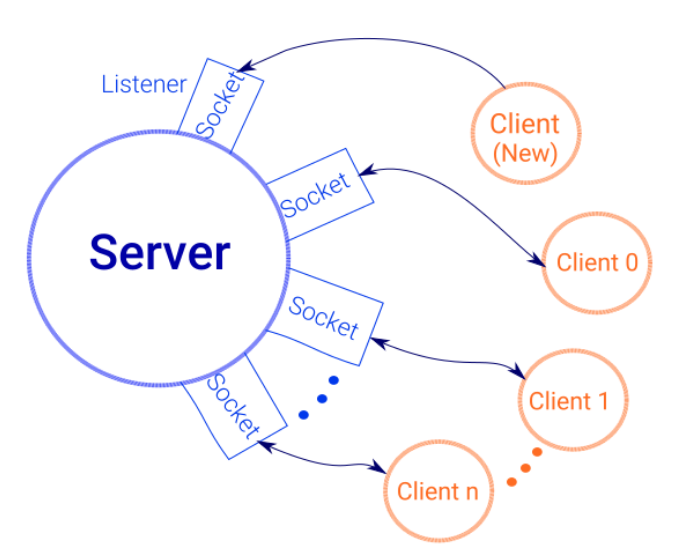
\includegraphics[scale=0.3]{socket.png}
  \caption{Взаимодействие клиента и сервера}\label{ris:socket}}
\end{figure}

\textbf{Сокет} --- абстрактный объект, представляющий конечную точку соединения. Сокет содержит в себе два параметра: IP---адрес и порт. Сервер, принимая соединение присваивает своему сокету определенный порт. Использовать порты с номерами 0 --- 1023 нельзя --- они зарезервированы под служебные сетевые протоколы (например, 21 --- FTP, 80 --- HTTP и т.д.). Клиент, отправляя данные тоже должен создать свой сокет. Два сокета с обоих сторон создают виртуальное соединение по которому будет идти передача данных. Нужно отметить, что при работе с протоколом TCP, создается два сокета: один из них — слушающий (listen). Он переходит в режим ожидания и активизируется при появлении нового соединения. При этом можно проверять актуальные активные соединения, установить периодичность операции. Второй — сокет для обмена данных с клиентом (accept).

В стандартной библиотеке python, существует модуль для работы с сетевым программированием. Что бы понять как работает TCP, расмотрим изображение~\ref{ris:TCP}.

\begin{figure}[h]
\center{\includegraphics[scale=0.3]{tcp.png}
  \caption{Протокол TCP}\label{ris:TCP}}
\end{figure}

Функция socket() инициализирует создание сокета. В ней передаются два параметра: communication domain и type of socket. По умолчанию передеается \verb!AF_INET! и \verb!SOCK_STREAM!. \verb!AF_INET! --- это коммуникационный домен, который задает сетевую направленность нашему сокету. Тип сокета --- \verb!SOCK_STREAM! он определяет сокет как потоковый, то есть реализующий последовательный, надежный двусторонний поток байтов по протоколу ТСР. Создалась конечная точка подключения --- сокет. Функция socket() возвращает нам файловый дескриптор, который позволяет работать с сокетом, как с файлом — записывать и считывать данные в/из него. Метод bind() присваевает порт, метод listen() устанавливает максимальное количество одновременных  запросов. Метод accept() подтверждает запрос на соединение и возвращает ip и адрес порта подключившегося клиента. Методы send() и recv() отправляют и получают сообщения. И наконец метод close() закрывает соединение.

Клиент устанавливает соединение с помощью метода connect (в нашем случае, localhost, т.к. сервер и клиент на одной машине). Как мы уже знаем, сервер отправляет нам последовательность кодированных байтов. Так же отправляет и получает сообщения методами send() и recv(). B закрывает соединение методом close()

Теперь перепишем приложение ``Список дел'' так что бы, сервер посылал клиенту данные из базы данных, затем клиент вносил изменения и посылал обратно на сервер при выключении приложения. Для этого необходимо разделить код на серверный код и клиентский.

На сервере оставляем работу с базой данных а все остальное переносим на клиент.

\lstinputlisting[caption='Сервер', language=Python]{todo_server.py}

\lstinputlisting[caption='Клиент', language=Python]{todo_client.py}


\newpage
\section{Задание на лабораторную работу}

Для выполнения работы необходимо:
\begin{enumerate}
  \item Изучить теоретический материал
%  \item Выбрать задание в соответствии с вариатом
  \item Добавить в ранее написаную программу работу в клиент-серверном режиме.
  \item Опубликовать код на github и предоставить ссылку в отчете
  \item Оформить отчет по лабораторной работе
\end{enumerate}

\section{Содержание отчета}
\begin{enumerate}
  \item Титульный Лист
  \item Цель работы
  \item Краткие теоретические сведения по теме лабораторной работы
  \item Выполненое задание
  \item Ссылка на github
  \item Краткий вывод о проделанной работе
\end{enumerate}

\begin{thebibliography}{3}
  \bibitem{python}Сузи, Р. А. Язык программирования Python : учебное пособие / Р. А. Сузи. — 3-е изд. — Москва : Интернет-Университет Информационных Технологий (ИНТУИТ), Ай Пи Ар Медиа, 2020. — 350 c. — ISBN 978-5-4497-0705-5. — Текст : электронный // Электронно-библиотечная система IPR BOOKS : [сайт]. — URL: http://www.iprbookshop.ru/97589.html
  \bibitem{tkinter} Документация стандартной библиотеки Python : socket — Python interface to Tcl/Tk [cайт]. --- URL: https://docs.python.org/3/library/socket.html
\end{thebibliography}


\end{document}
